% !TeX root = ExtendedAbstract.tex

\section{Persistence Homology}

\nocite{polterovich}

Persistence homology is a tool developed around 1992 for the purpose of data science. Data scientists had the need to compute the homology of a shape given a finite collection of data points $X$, which raises the question of finding a shape which adequately describes the data. A primitive algorithm consists of picking a positive number $r$ and replacing each data point by a sphere of radius $r$. The resulting open set, denoted $X^{(r)}$, may be understood as an approximation of the real shape underlying the data $X$, and there are efficient algorithms to compute its homology.

\begin{figure}
\centering
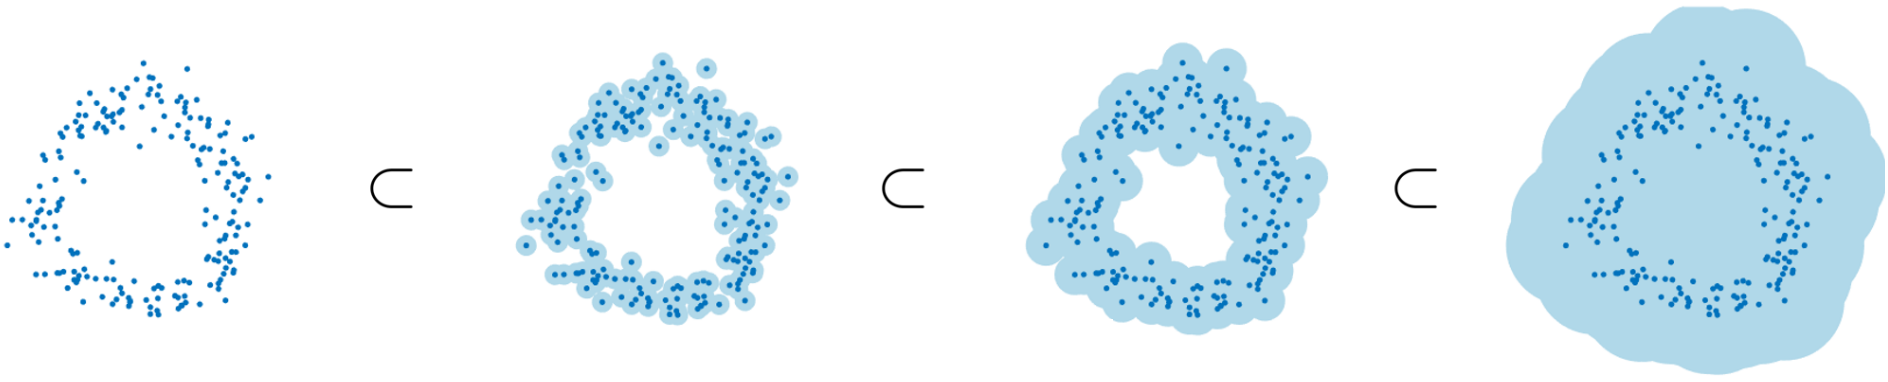
\includegraphics[width=\linewidth]{data}
\caption{Illustration of the sets $X^{(r)}$, with increasing $r$. Note that the middle radii are the ones which better represent the topology of the data. Figure taken from \cite{historypersistence}.}
\end{figure}

This raises the question of which radius $r$ to pick, which requires careful analysis of the data: too small $r$ and the datapoints will be disconnected, too large $r$ and the dataset degenerates into a large ball. However, persistence homology offers an alternative: consider all positive radii at once.

For $k \in \Z$ and $r > 0$, define $H_k^r(X) = H_k(X^{(r)})$, and for $r \leq 0$ set $H_k^r(X) = 0$. These spaces allow us to visualize how the shape of $X^{(r)}$ changes as $r$ increases. Moreover, for $r < s$ the inclusion $X^{(r)} \subseteq X^{(s)}$ induces a natural map $H_k^r(X) \to X_k^s(X)$. This data forms an object which is called a \emph{persistence module}. In the sequence we will be working exclusively with vector spaces, so assume that the homology is taken with coefficients over a field $\FF$.

\begin{definition}
A persistence module is a family of vector spaces $\{V_t\}_{t \in \R}$ (over a field $\FF$), together with maps $\pi_{st} \colon V_s \to V_t$ for $s \leq t$, such that
\begin{align}
\pi_{tt} &= \id,\\
\pi_{tr} \circ \pi_{st} &= \pi_{sr}, \quad s \leq t \leq r.
\end{align}

Moreover, a persistence module $(\{V_t\}_{t \in \R}, \{\pi_{st}\}_{s\leq t})$ is said to be of \emph{finite type} if the following three conditions are satisfied:
\begin{enumerate}
\item For all but finitely many $t$ there exists a neighborhood $U$ of $t$ such that $\pi_{st}$ is an isomorphism for $s, t \in U$,
\item For all $t \in \R$ there exists $\varepsilon$ such that $\pi_{(t-\delta), t}$ is an isomorphism for all $0 \leq \delta < \varepsilon$,
\item\label{pm3} For all $t \in \R$ close enough to $-\infty$, $V_t = 0$.
\end{enumerate}
\end{definition}

In practice, all the constructions for persistence modules that will be discussed in this thesis originate persistence modules of finite type. This is useful because of an important representation theorem for this class of persistence modules. We now introduce the relevant concepts.

\begin{definition}
A \emph{barcode} is a finite multiset\footnote{A multiset is a set whose elements are counted with multiplicity.} of intervals of type $\linterval a b$, with $-\infty < a < b \leq +\infty$. We work under the convention that $\linterval a \infty = \ointerval a \infty$.
\end{definition}

\begin{definition}
Let $B = \{I_1, \dots, I_n\}$ be a barcode. Define the persistence module $\FF(B) = (\{V_t\}_{t \in \R}, \{\pi_{st}\}_{s \leq t})$ as follows
\begin{itemize}
\item Define $V_t = \braket{\,i \mid t \in I_i\,}$, where the brackets denote the free vector space over $\FF$,
\item For $s \leq t$, define $\pi_{st} \colon V_s \to V_t$ by defining it on the basis elements of $V_s$. For every $i$ such that $s \in I_i$,
\begin{itemize}
\item If $t \in I_i$, set $\pi_{st}(i) = i$,
\item Otherwise, set $\pi_{st}(i) = 0$.
\end{itemize}
\end{itemize}

It is straight-forward to prove that $\FF(B)$ is a persistence module of finite type.
\end{definition}

\begin{theorem}[Normal Form Theorem]
Every persistence module of finite type is isomorphic to $\FF(B)$ for exactly one barcode $B$.
\end{theorem}

The normal form theorem is the persistence analogous to the classical theorem in linear algebra that says that every vector space of finite dimension is isomorphic to $\R^n$ for some unique $n$. By property \ref{pm3} of finite type persistence modules, every persistence module `starts out' as the zero vector space, and at some instant in time it `grows a new basis element'. This marks the start of a bar in its barcode. Similarly, whenever the vector space $V_t$ loses a dimension, that is marked by the end of a bar. In this sense, the barcode of a persistence module is an indicator of when dimensions are appearing and disappearing; when applied to the homology of a topological space, \emph{the bars mark the appearance and disappearance of holes in the space as the parameter varies}.

[[Torus example here maybe?]]


\section{Floer Homology}
\label{sec:ph}

Floer homology was developed by Andreas Floer in 1988 in order to attack the so-called Arnol'd conjecture, an important problem in symplectic geometry.

Floer homology can be seen as an analogue of Morse homology happening in contractible loop space, so the reader who is already familiar with Morse theory will want to read the following with that in mind.

